To install and run our software it is necessary to download Ultimate IntellJ Idea and docker. By using docker we have been able to cancel the whole process of downloading, installing and setting both server and database; both are simulated in dockers defined in the dockerfile.

\section{Linux - Fedora}
We have worked on Fedora 29, the following instructions, especially for what is related to Docker, are strictly related to this Linux platform.\\
The following steps are necessary to correctely run our software on Fedora:
\begin{itemize}
	\item Download the \textbf{Ultimate IntellJ} version which can be found at the following link:\\
 		\url{https://www.jetbrains.com/idea/download/#section=windows}

	\item Download \textbf{Android Studio} for simulate the two clients, the latest version can be found at the following link:\\
		\url{https://developer.android.com/studio/}
		To correctly install this software follow the steps at the following link:\\
		\url{https://developer.android.com/studio/intro/}

	\item For docker follow the prompt command explained in the next link:\\
		\url{https://developer.fedoraproject.org/tools/docker/docker-installation.html}\\


	\item To run the server code the following prompt commands must be executed:\\
		\begin{itemize}
			\item \textbf{selinux} and then \textbf{sudo setenforce 0}: to disactivate the security and let docker work;
			\item \textbf{sudo dnf install docker docker-compose}: to install the docker compose package;
			\item \textbf{sudo groupadd docker \&\& sudo gpasswd -a \${USER} docker}
			\item \textbf{newgrp docker}
			\item \textbf{ mvn clean install -DskipTests} : to correctly build the maven project;
			\item \textbf{ sudo systemctl start docker} : because of the sudo command it will be necessary to confirm the 					command by inserting the password. This command is fundamental to start up the docker deamon,	
			\item \textbf{ docker-compose up - -build} : to build the docker which will contain the container for both server 					and DB.\\N:B The space between - - is incorrect, here it has been added jsut to show the presence of two - -.
		\end{itemize}

	\item Before starting the client it is necessary to create the DataSource in server by folowing the next fw steps:
	\begin{figure}[h!]
		\centering
		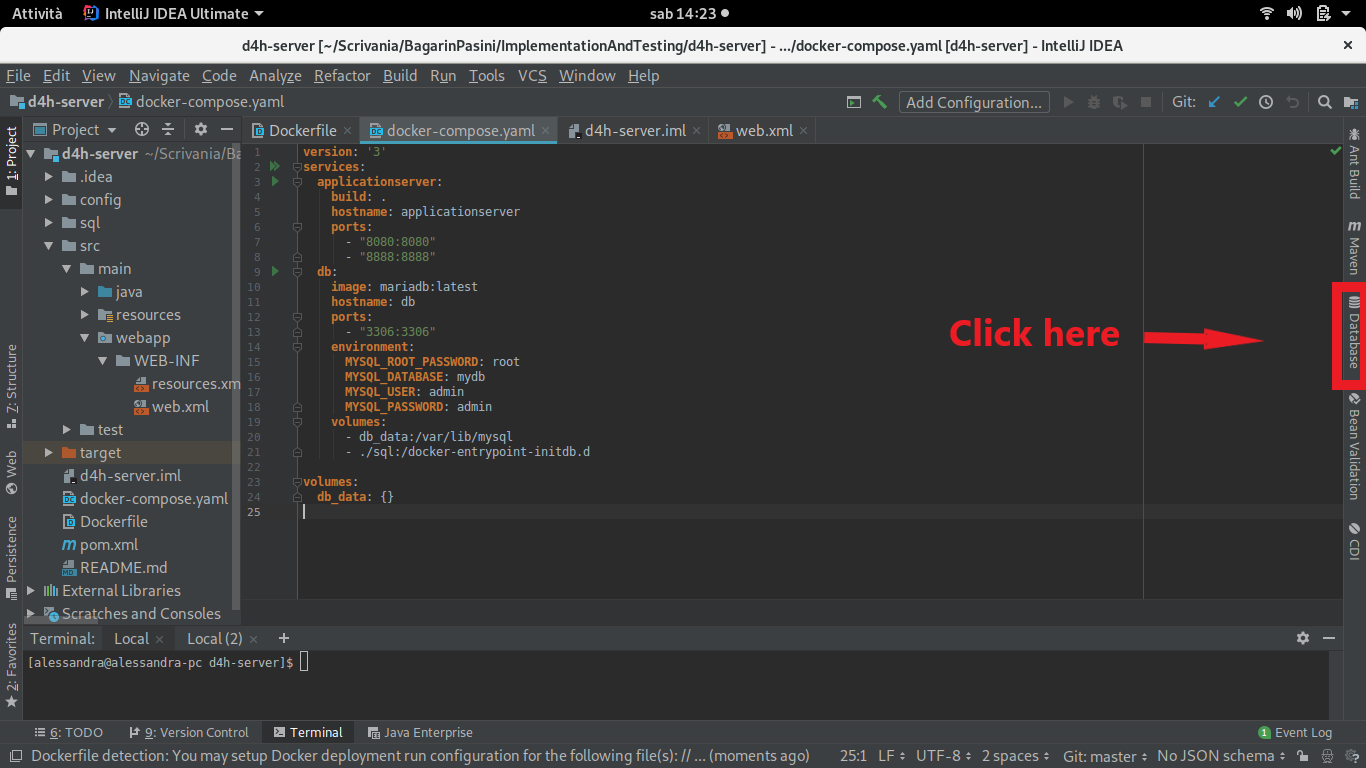
\includegraphics[width=1.0\textwidth]{./pictures/first_step.png}\par
		\caption{Click on the database button in the right side of IntellJ Ultimate}
	\end{figure}
	\FloatBarrier
	\begin{figure}[h!]
		\centering
		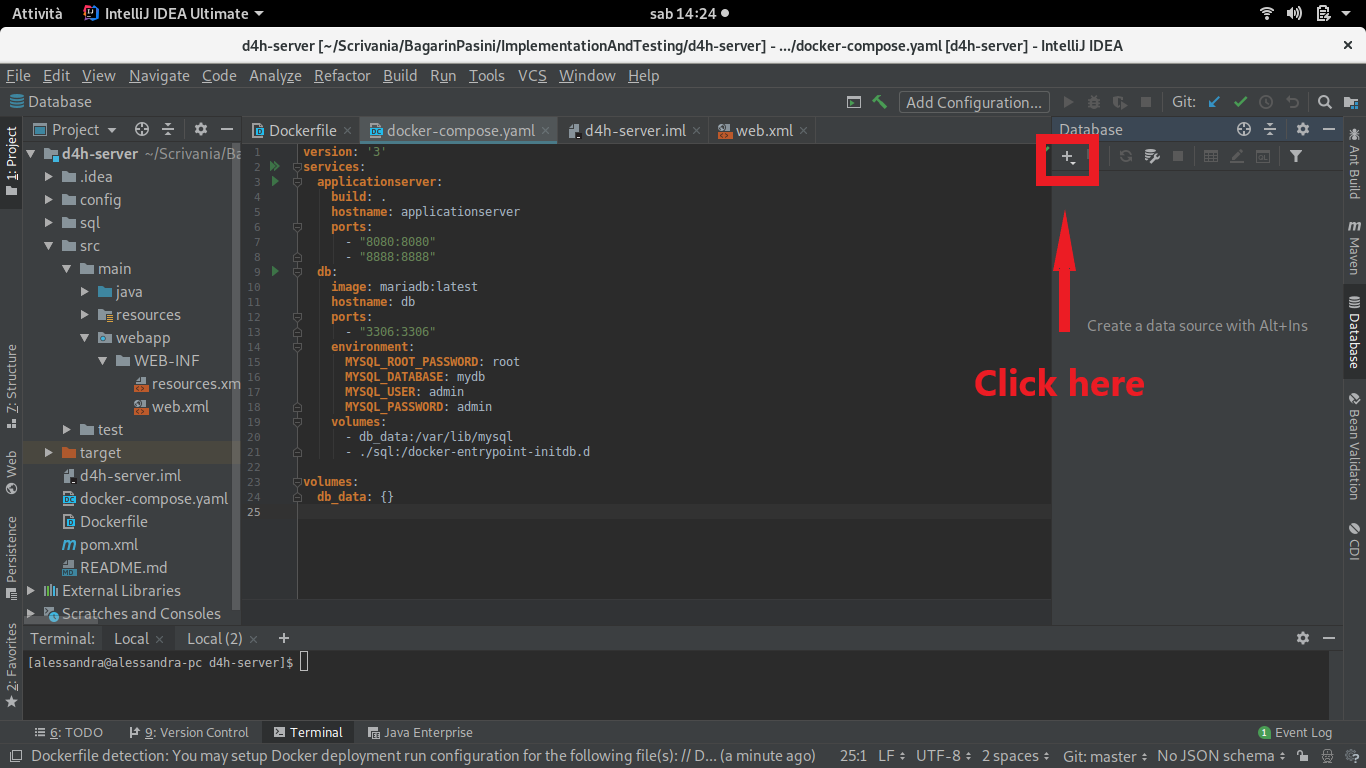
\includegraphics[width=1.0\textwidth]{./pictures/second_step.png}\par
		\caption{Click on the plus button to add a new DataSource. Select DataSource, click on MariaDB. }
	\end{figure}
	\FloatBarrier
	\begin{figure}[h!]
		\centering
		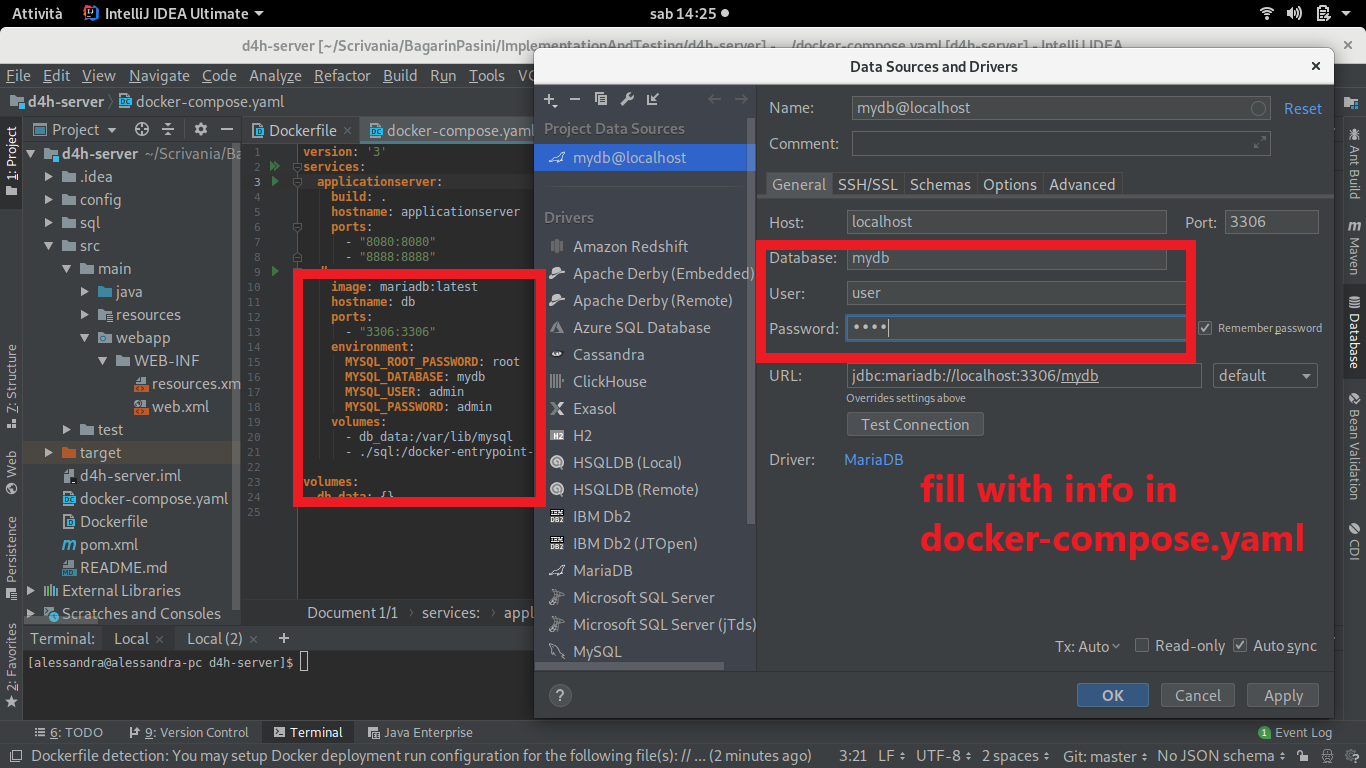
\includegraphics[width=1.0\textwidth]{./pictures/third_step.png}\par
		\caption{Fill the properties.}
	\end{figure}
	\FloatBarrier
	\begin{figure}[h!]
		\centering
		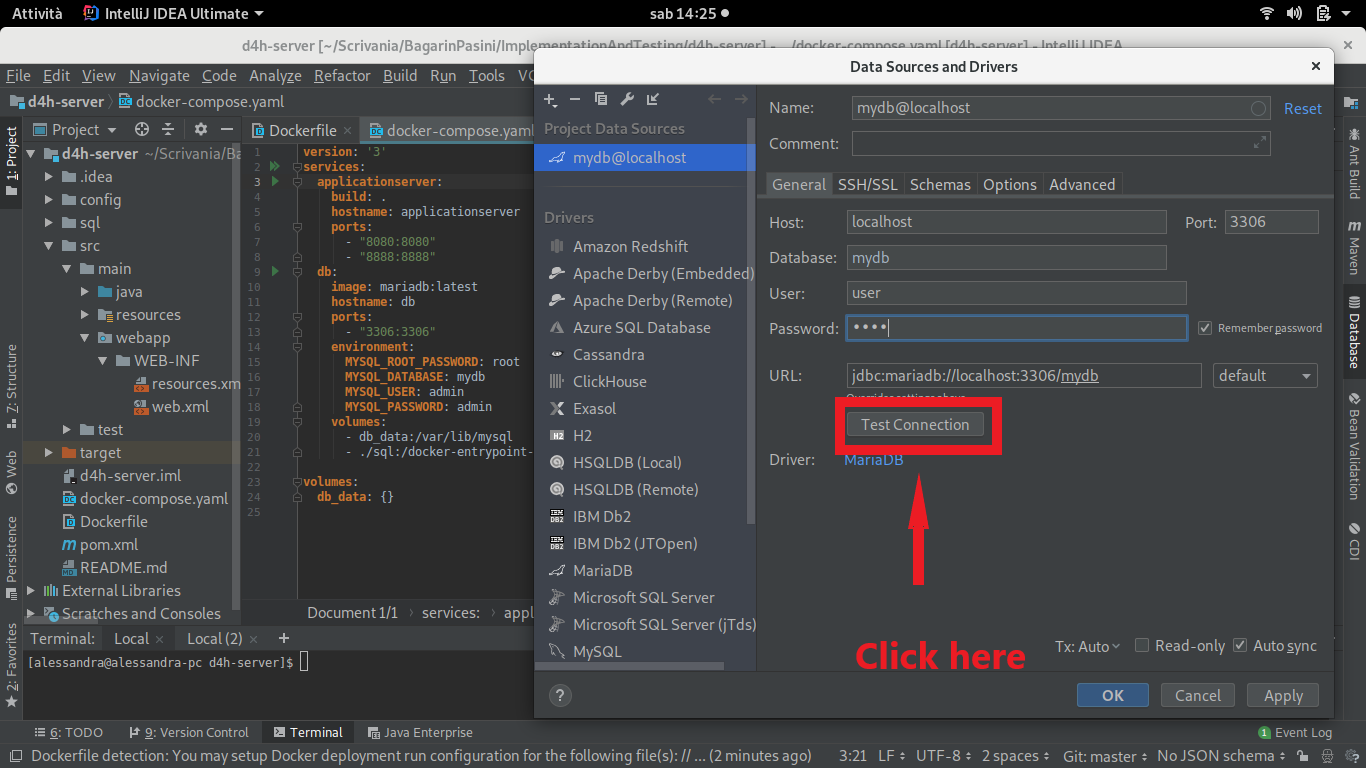
\includegraphics[width=1.0\textwidth]{./pictures/fourth_step.png}\par
		\caption{Once all properties are added verify if the connection has been established in a correct way. The test should be successful because the docker has already been built up.}
	\end{figure}
	\FloatBarrier
	\begin{figure}[h!]
		\centering
		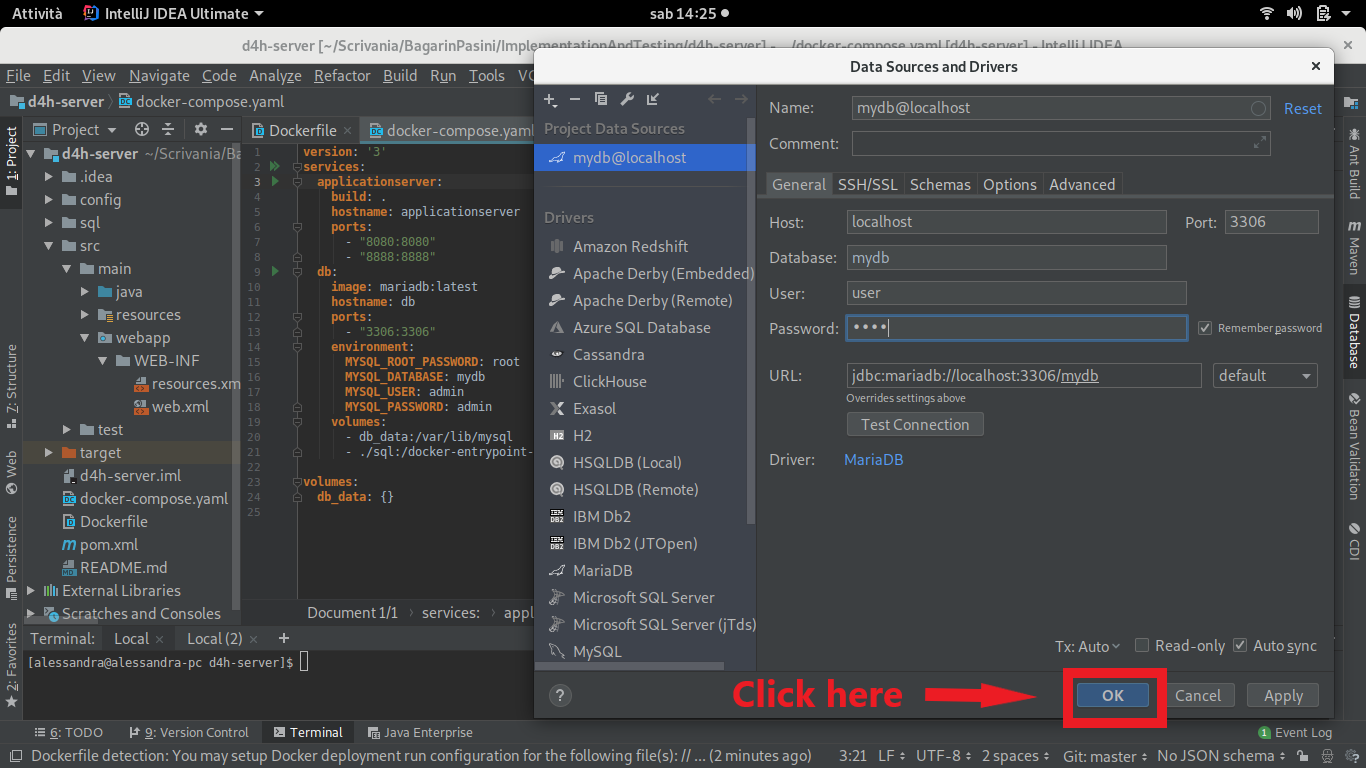
\includegraphics[width=1.0\textwidth]{./pictures/fifth_step.png}\par
		\caption{Click okey to build the DataSource.}
	\end{figure}
	\FloatBarrier

	\item To run the client code it is necessary to:
		\begin{itemize}
			\item go in \textit{config.class} and modify the domain in URL string (of course it will have to be the domain on 					which the server works);
			\item go in the \textit{networksecurityconfig.xm}l to modify the URL string as in config.class.
			\item run the app on an emulator phone.
		\end{itemize} 
\end{itemize}
More details can be found in the server's ReadMe which includes some more docker commands that might be useful in case of problems, such as having some dockers that already work on the prefixed doors 8080 and 3306.

\section{Windows}
The following steps are necessary to correctely run our software on Fedora:
\begin{itemize}
	\item Download the \textbf{Ultimate IntellJ} version which can be found at the following link:\\
 		\url{https://www.jetbrains.com/idea/download/\#section=windows}

	\item Download \textbf{Android Studio} for simulate the two clients, the latest version can be found at the following link:\\
		\url{https://developer.android.com/studio/}

		To correctly install this software follow the steps at the following link:\\
		\url{https://developer.android.com/studio/intro/}

	\item To correctly download and install docker follow the instruction explained in the folowing link:\\
		\begin{itemize}
		\item if you have Windows 10 Pro, Education, Enterprise download it at: \url{https://docs.docker.com/docker-for-					windows/install/}\\
		\item if you have lower versions download it at \url{https://docs.docker.com/toolbox/toolbox_install_windows/}
		\end{itemize}
	When installing the docker remember that you will need to install also the docker-compose which is give for free in Windows 			and OS docker installation.

	\item To run the server code the following prompt commands must be executed:\\
		\begin{itemize}
			\item To run the  Maven project by using the Maven Docker image directly, pass a Maven command to docker 					run:\\
\textit{\$ docker run -it --rm --name my-maven-project -v "\$(pwd)":/usr/src/mymaven -w /usr/src/mymaven maven:3.3-jdk-8 mvn clean install -DskipTests};
			\item \textbf{start docker}this command is fundamental to start up the docker deamon;	
			\item \textbf{ docker-compose up - -build} : to build the docker which will contain the container for both server 					and DB.\\N:B The space between - - is incorrect, here it has been added jsut to show the presence of two - -.
		\end{itemize}

	
	\item To run the client code it is necessary to:
		\begin{itemize}
			\item go in \textit{config.class} and modify the domain in URL string (of course it will have to be the domain on 					which the server works);
			\item go in the  \textit{networksecurityconfig.xml}  to modify the URL string as in config.class.
			\item run the app on an emulator phone.
		\end{itemize} 
\end{itemize}

\subsection{Mac OS}
The following steps are necessary to correctely run our software on Fedora:
\begin{itemize}
	\item Download the \textbf{Ultimate IntellJ} version which can be found at the following link:\\
 		\url{https://www.jetbrains.com/idea/download/#section=windows}

	\item Download \textbf{Android Studio} for simulate the two clients, the latest version can be found at the following link:\\
		\url{https://developer.android.com/studio/}

		To correctly install this software follow the steps at the following link:\\
		\url{https://developer.android.com/studio/intro/}

	\item To run the server code the following prompt commands must be executed:\\
	
		\begin{itemize}
			\item To run the  Maven project by using the Maven Docker image directly, pass a Maven command to docker 					run:\\
\textit{\$ docker run -it --rm --name my-maven-project -v "\$(pwd)":/usr/src/mymaven -w /usr/src/mymaven maven:3.3-jdk-8 mvn clean install -DskipTests};
			\item \textbf{ sudo systemctl start docker} : because of the sudo command it will be necessary to confirm the 					command by inserting the password. This command is fundamental to start up the docker deamon,	
			\item \textbf{ docker-compose up - -build} : to build the docker which will contain the container for both server 					and DB.\\N:B The space between - - is incorrect, here it has been added jsut to show the presence of two - -.
		\end{itemize}

	
	\item To run the client code it is necessary to:
		\begin{itemize}
			\item go in \textit{config.class} and modify the domain in URL string (of course it will have to be the domain on 					which the server works);
			\item go in the  \textit{networksecurityconfig.xml}  to modify the URL string as in config.class.
			\item run the app on an emulator phone.
		\end{itemize} 
\end{itemize}

For more details on Docker and Docker compose look at this link:\\
\url{https://docs.docker.com/}
